\clearpage
\section*{Supplementary Figures}
\begin{figure}[ht]
\centering
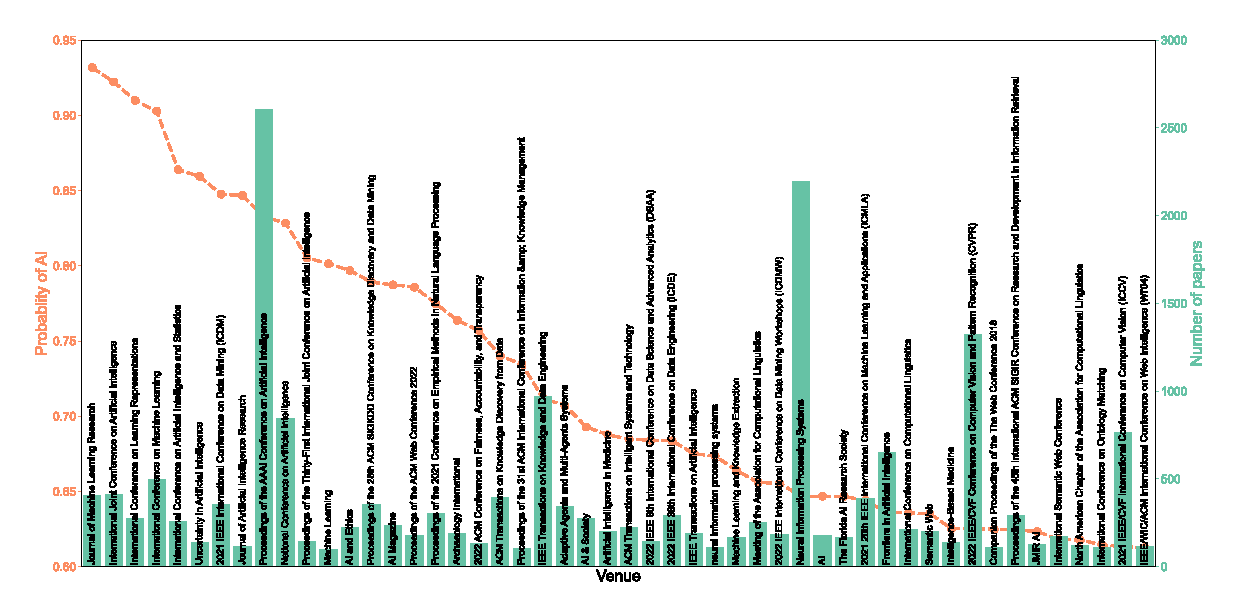
\includegraphics[width=\textwidth]{figure_SI/S1.pdf}
\caption{
\textbf{Probability of AI (orange) and number of papers (green) for selected venues.} 
Final identification results combine the best models in both stages of fine-tuning. Venues are ordered according to the probability of AI papers within them.
}
\label{figs1}
\end{figure}


\clearpage
\newpage
\begin{figure}[ht]
\centering
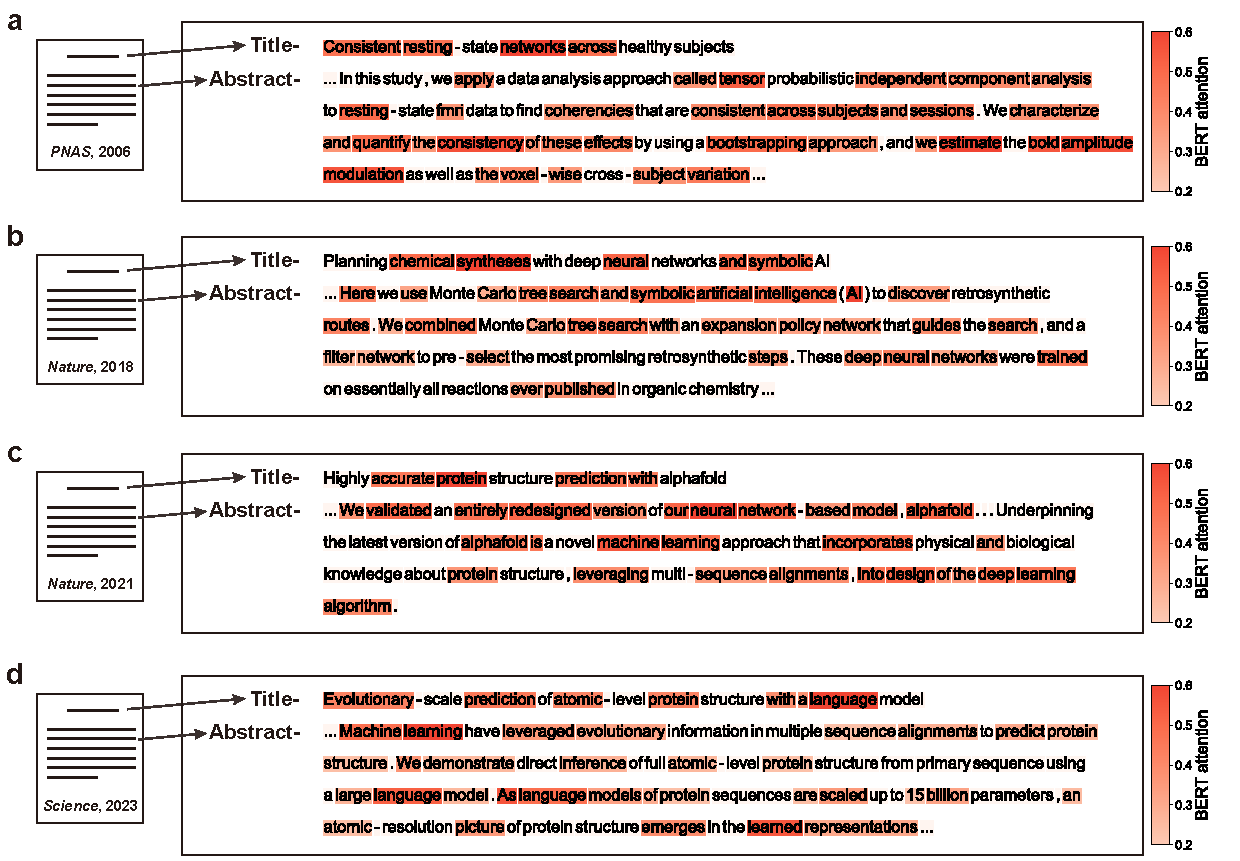
\includegraphics[width=\textwidth]{figure_SI/R1S14a.pdf}
\caption{\textbf{Correct examples of AI paper identification across different eras of AI development.}
\textbf{(a)} Example from the ML era, a medicine paper with AI published in \textit{PNAS} 2006.
\textbf{(b)} Example from the DL era, a chemistry paper with AI published in \textit{Nature} 2018.
\textbf{(c)} Example from the DL era, a biology paper with AI published in \textit{Nature} 2021.
\textbf{(d)} Example from the GAI era, a biology paper with AI published in \textit{Science} 2023.
}
\label{figsR1S14a}
\end{figure}

\clearpage
\newpage
\begin{figure}[ht]
\centering
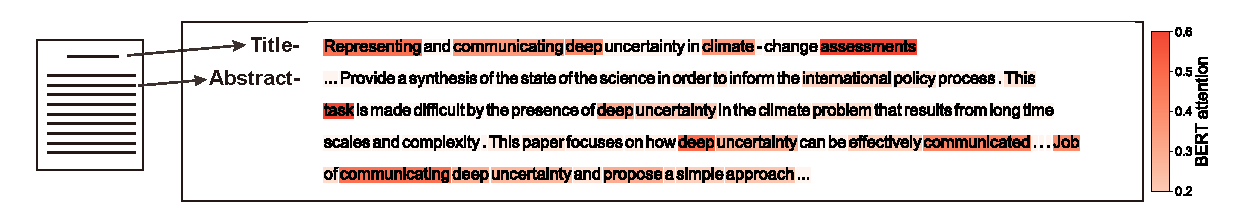
\includegraphics[width=\textwidth]{figure_SI/R1S14b.pdf}
\caption{
\textbf{An incorrect example of AI paper identification.}
The example is a geology paper without AI published in 2006, which is mistaken to be AI-related by the identification model.
}
\label{figsR1S14b}
\end{figure}


\clearpage
\newpage
\begin{figure}[ht]
\centering

\includegraphics[width=\textwidth]{figure_SI/S4.pdf}
\caption{
\textbf{Topics with top occurrence frequency in AI and non-AI papers.}
Results show that AI’s primary contribution to conventional research fields is around computer science and machine learning algorithms.
Across disciplines, identified AI papers turn out to be selected combinations of conventional research topics and AI-related techniques, including “Artificial Intelligence”, “Computer Vision and Pattern Recognition”, and “Computational Theory and Mathematics”. 
}
\label{figs3}
\end{figure}


\clearpage
\newpage
\begin{figure}[ht]
\centering
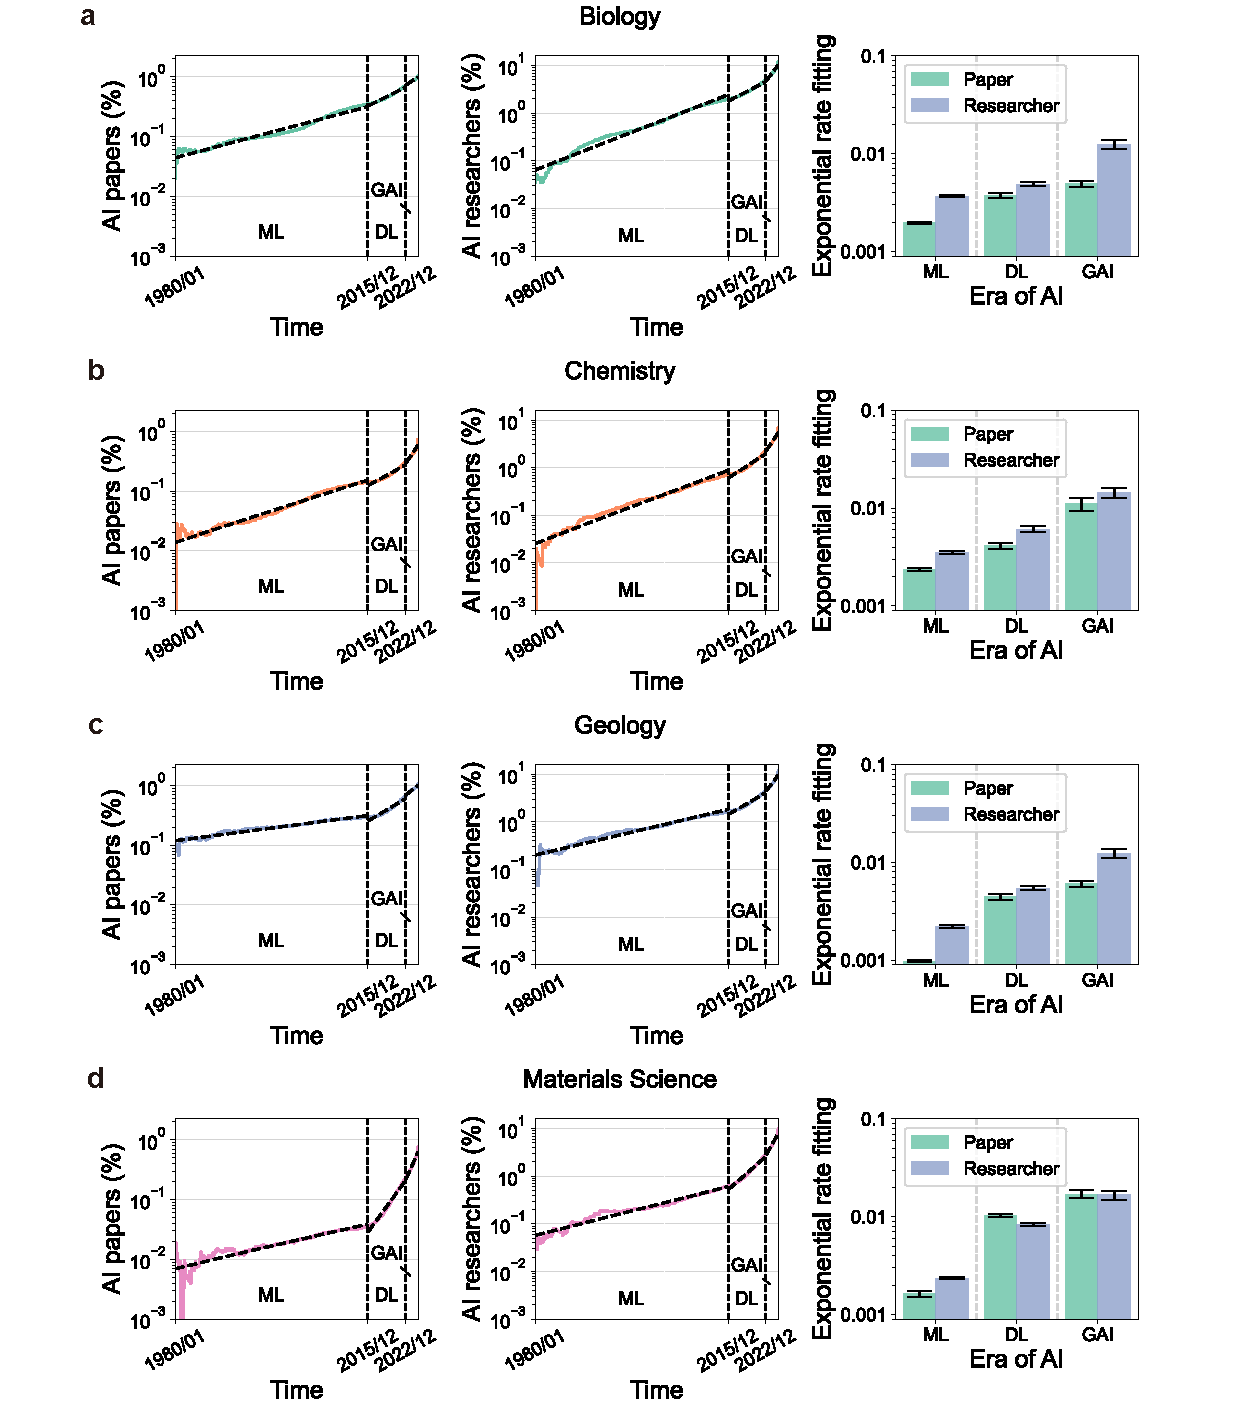
\includegraphics[width=\textwidth]{figure_SI/R1S12a.pdf}
\caption{
\textbf{Proportion of papers and researchers adopting AI in each discipline with log-scale y-axis and estimated growth rate with exponential fitting for each era.}
Proportion of papers and researchers adopting AI fit to straight regions in the log-scale plot, indicating high precision of the exponential fitting.
Meanwhile, estimated by the exponential fitting, the growth rate of AI papers and AI researchers in all disciplines increased progressively from the ML era to the DL and GAI eras.
For the estimated growth rates ($n=543$ month observations), 99\% CIs are shown as error bars centred at the mean.
}
\label{figsR1S12a}
\end{figure}

\clearpage
\newpage
\begin{figure}[ht]
\centering
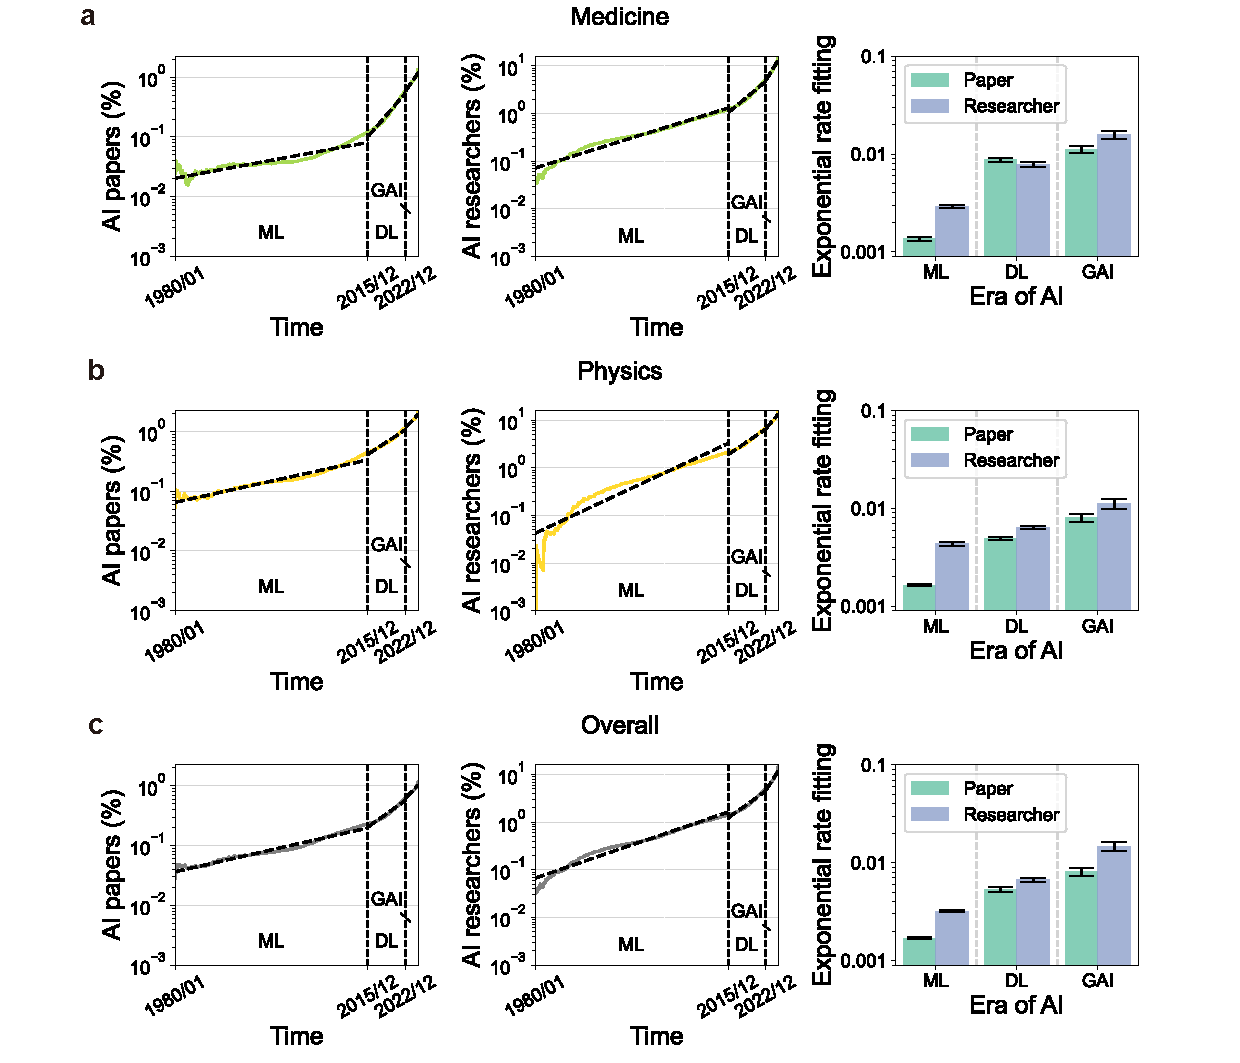
\includegraphics[width=\textwidth]{figure_SI/R1S12b.pdf}
\caption{
\textbf{(Continued from Supplementary Fig.~S\ref{figsR1S12a}) The proportion of papers and researchers adopting AI in each discipline with log-scale y-axis and estimate the growth rate with exponential fitting in each era.}
The proportion of papers and researchers adopting AI fit to straight regions in the log-scale plot, indicating high precision of the exponential fitting.
Meanwhile, estimated by the exponential fitting, the growth rate of AI papers and AI researchers in all disciplines increased progressively from the ML era to the DL and GAI eras.
For the estimated growth rates ($n=543$ month observations), 99\% CIs are shown as error bars centred at the mean.
}
\label{figsR1S12b}
\end{figure}

\clearpage
\newpage
\begin{figure}[ht]
\centering
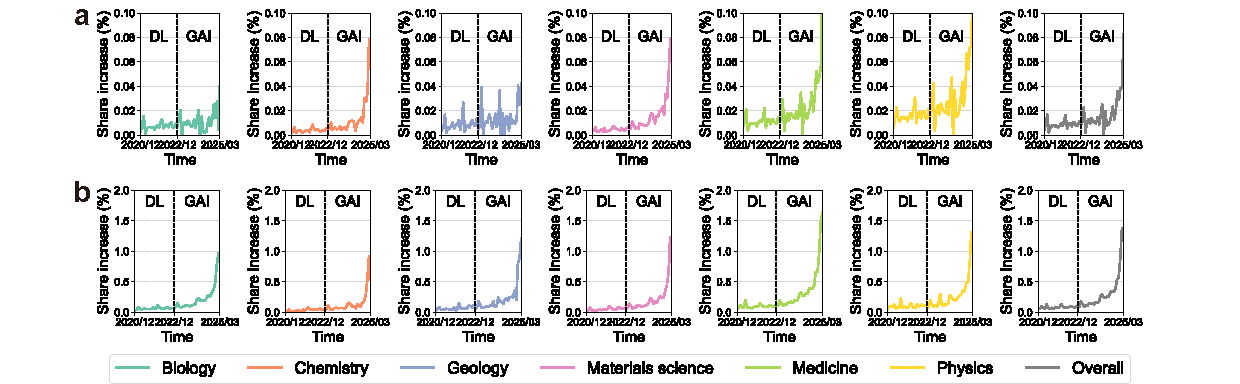
\includegraphics[width=\textwidth]{figure_SI/R1S13.pdf}
\caption{
\textbf{The monthly increase in the proportion of AI (a) papers and (b) researchers across disciplines in recent years.}
Following the release of ChatGPT in December 2022, growth rates in the proportion of papers and researchers initially remain consistent with prior trends.
A period of time later, these growth rates begin to exhibit a marked acceleration across disciplines, providing evidence for the impact of generative AI advancement and use.
}
\label{figsR1S13}
\end{figure}

\clearpage
\newpage
\begin{figure}[ht]
\centering
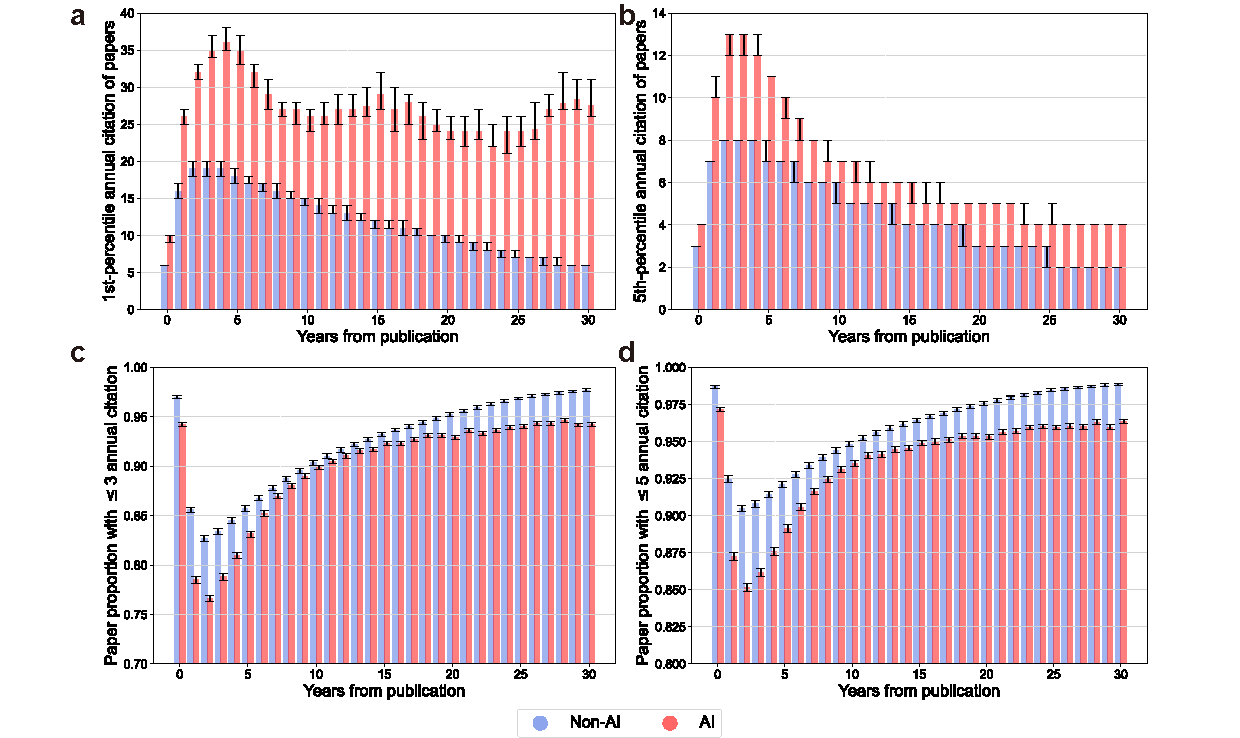
\includegraphics[width=\textwidth]{figure_SI/R1S4.pdf}
\caption{
\textbf{Alternative statistical indicators for the annual citation comparison between AI and non-AI papers.}
\textbf{(a)} Top 1st-percentile annual citation for AI and non-AI papers from year of publication ($n=27,405,011$).
\textbf{(b)} Top 5th-percentile annual citation for AI and non-AI papers from year of publication ($n=27,405,011$).
\textbf{(c)} Proportion of AI and non-AI papers receiving fewer than three citations each year from year of publication ($n=27,405,011$).
\textbf{(d)} Proportion of AI and non-AI papers receiving fewer than five citations each year from year of publication ($n=27,405,011$).
For all panels, 99\% CIs are shown as error bars centred at the corresponding percentiles or proportions.
}
\label{figsR1S4}
\end{figure}

\clearpage
\newpage
\begin{figure}[ht]
\centering
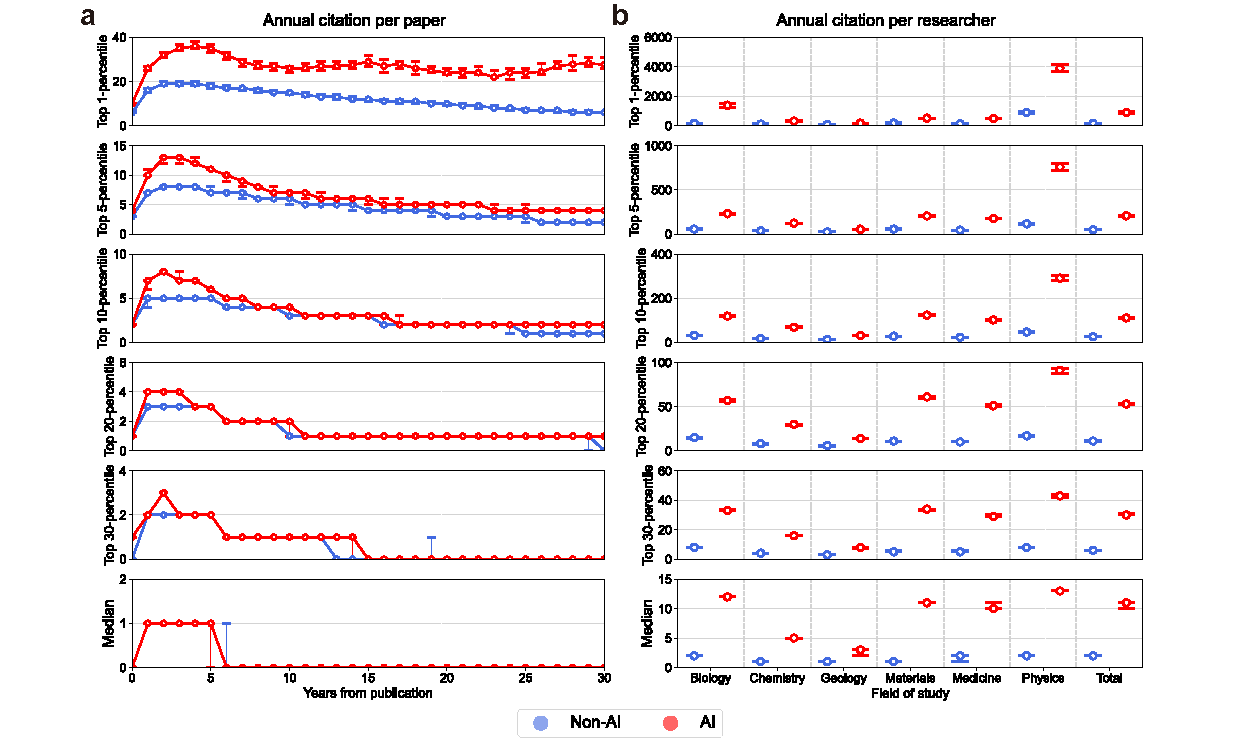
\includegraphics[width=\textwidth]{figure_SI/R2S4.pdf}
\caption{
\textbf{Different percentile statistics for the annual citation comparison between AI and non-AI papers.}
\textbf{(a)} Annual citations after publication of AI and non-AI papers ($n=27,405,011$).
\textbf{(b)} Annual citations for researchers adopting AI and their counterparts without AI ($n=5,377,346$).
Consistently indicated by different percentile statistics, AI papers and researchers attract more citations.
For all panels, 99\% CIs are shown as error bars centred at the corresponding percentiles.
}
\label{figsR2S4}
\end{figure}

\clearpage
\newpage
\begin{figure}[ht]
\centering
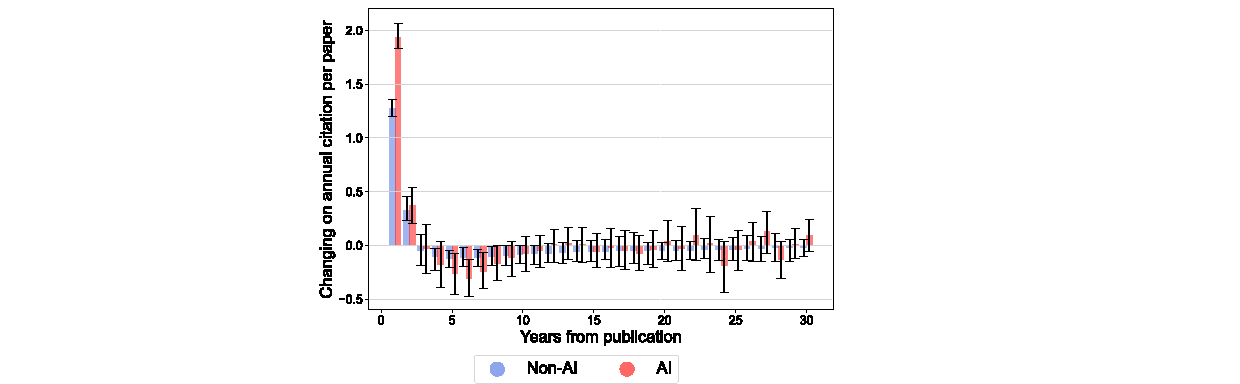
\includegraphics[width=\textwidth]{figure_SI/R1S3.pdf}
\caption{
\textbf{Comparison of “acceleration” of citation, namely year-over-year change in annual citation counts, between AI and non-AI papers.}
AI papers experience a faster acceleration in citation growth during the initial post-publication years, and exhibit a more rapid deceleration in annual citations after reaching peak annual citations ($n=27,405,011$).
Throughout the entire citation lifecycle, the annual citation of AI papers consistently remains higher than that of non-AI papers.
99\% CIs are shown as error bars centred at the mean.
}
\label{figsR1S3}
\end{figure}

\clearpage
\newpage
\begin{figure}[ht]
\centering
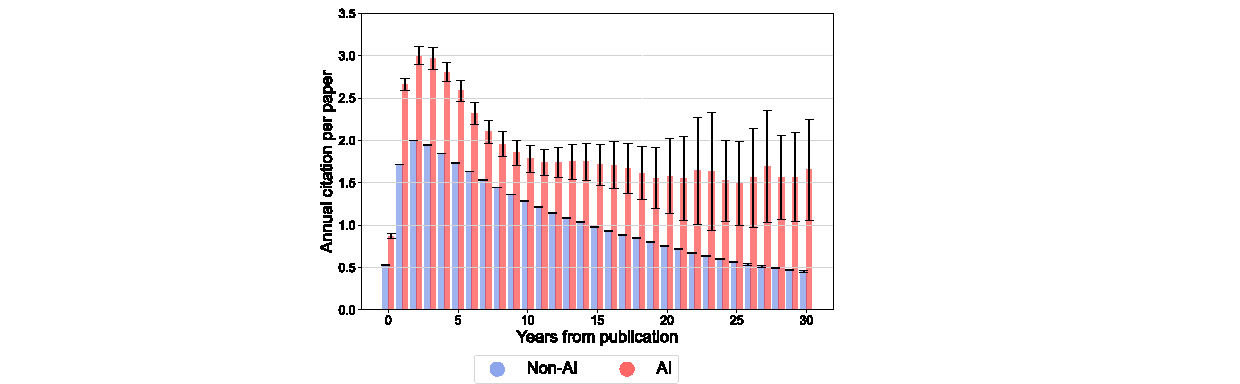
\includegraphics[width=\textwidth]{figure_SI/R1S5a.pdf}
\caption{
\textbf{Annual citations after the publication of AI and non-AI original research papers, excluding review articles, editorial pieces and other special publications.}
Results show that AI papers attract more citations, indicating higher academic impact than papers without AI ($n=24,867,012$).
Results are consistent with the overall statistics in the main text.
99\% CIs are shown as error bars centred at the mean.
}
\label{figsR1S5a}
\end{figure}

\begin{figure}[ht]
\centering
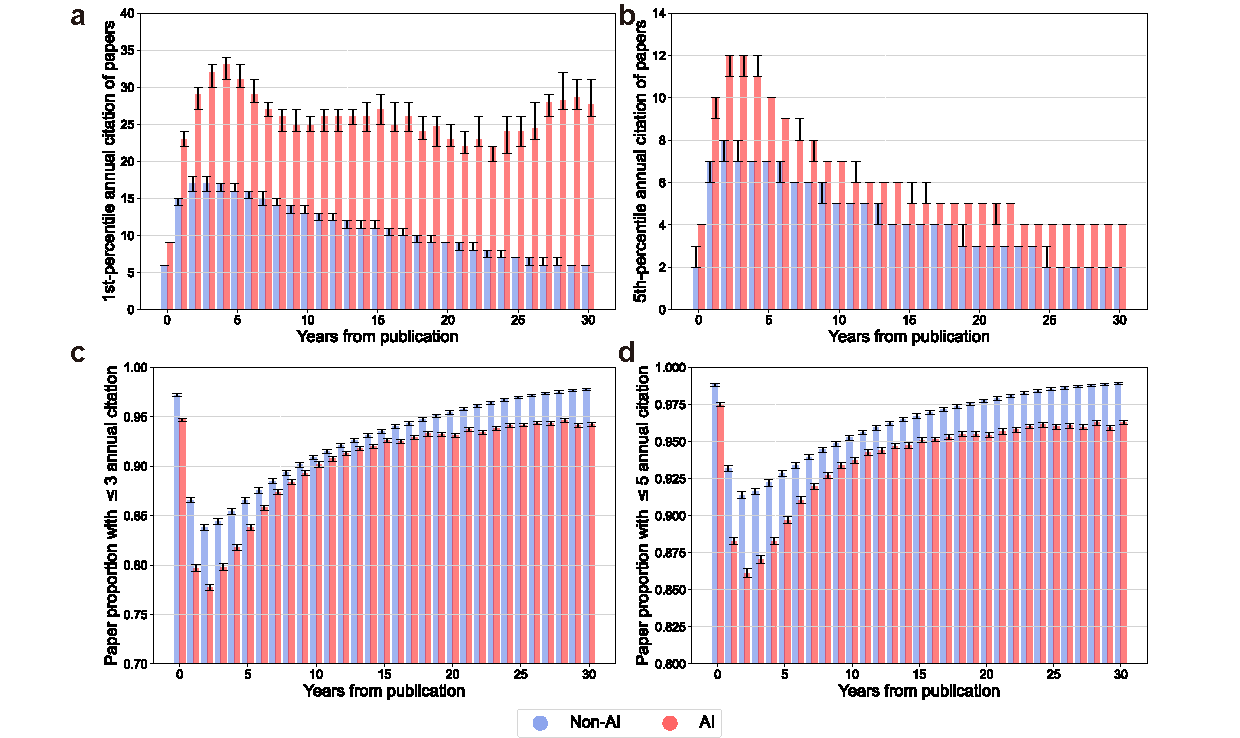
\includegraphics[width=\textwidth]{figure_SI/R1S5b.pdf}
\caption{
\textbf{Alternative statistical indicators for the annual citation comparison between AI and non-AI original research papers, excluding review articles, editorial pieces and other special publications.}
\textbf{(a)} Top 1st-percentile annual citation for AI and non-AI papers from year of publication ($n=24,867,012$).
\textbf{(b)} Top 5th-percentile annual citation for AI and non-AI papers from year of publication ($n=24,867,012$).
\textbf{(c)} Proportion of AI and non-AI papers receiving fewer than three citations each year from year of publication ($n=24,867,012$).
\textbf{(d)} Proportion of AI and non-AI papers receiving fewer than five citations each year from year of publication ($n=24,867,012$).
Results are consistent with the overall statistics in the main text.
For all panels, 99\% CIs are shown as error bars centred at the mean.
}
\label{figsR1S5b}
\end{figure}

\clearpage
\newpage
\begin{figure}[ht]
\centering
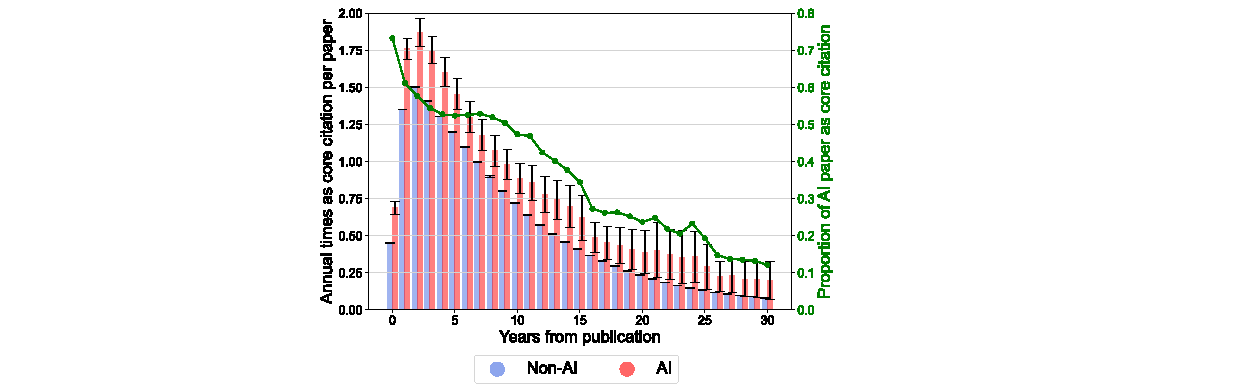
\includegraphics[width=\textwidth]{figure_SI/R1S8.pdf}
\caption{
\textbf{Distinguishing between core and superficial citations.}
Results show that the proportion of AI papers cited as core citations tends to decrease over time (green line), while foundational influence can still be observed in decades-old papers ($n=27,405,011$).
In terms of the absolute count of instances being among the core citations in future papers, AI papers still outperform non-AI papers (red and blue bars), reflecting their enhanced academic impact. 
99\% CIs are shown as error bars centred at the mean.
}
\label{figsR1S8}
\end{figure}

\clearpage
\newpage
\begin{figure}[ht]
\centering
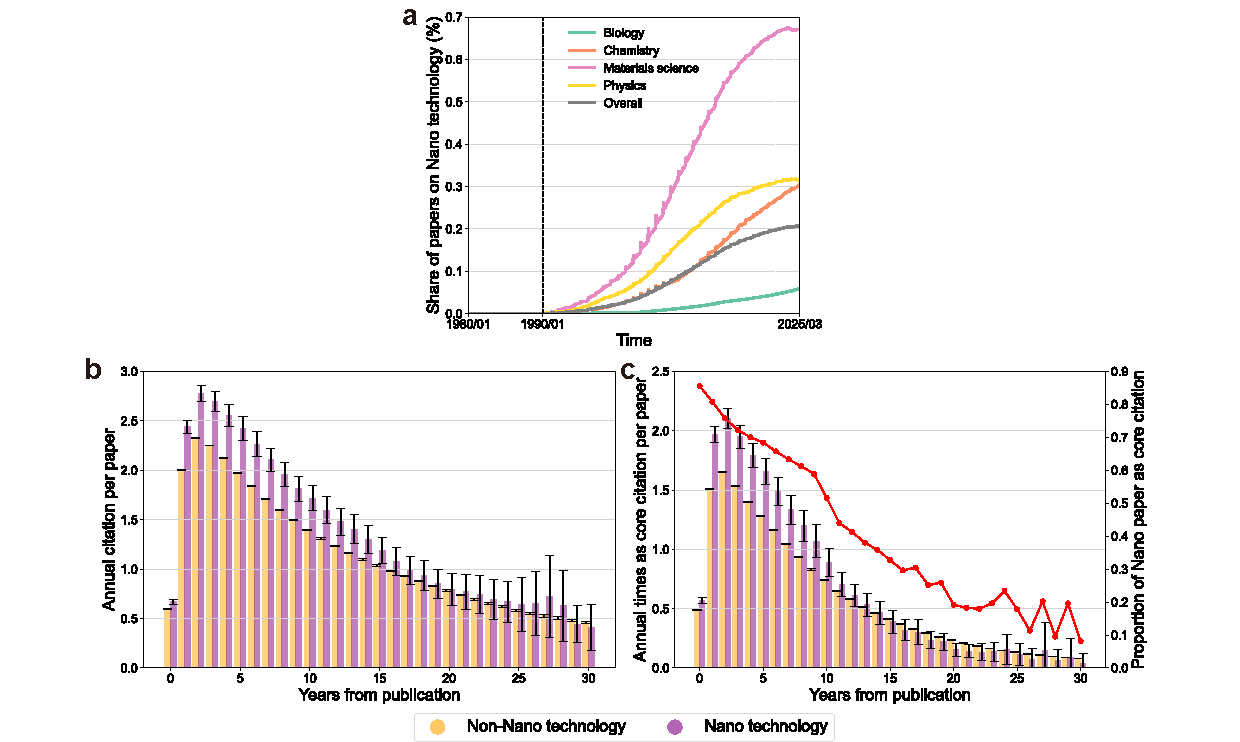
\includegraphics[width=\textwidth]{figure_SI/R1S9.pdf}
\caption{
\textbf{Comparison between citation patterns of Nanotechnology and non-Nanotechnology papers.}
\textbf{(a)} Growth of Nanotechnology over time in different disciplines.
\textbf{(b)} Annual citations after publication of Nanotechnology and non-Nanotechnology papers ($n=17,976,303$).
\textbf{(c)} Annual times of being core citation following publication of Nanotechnology and non-Nanotechnology papers ($n=17,976,303$).
Nanotechnology papers are still cited as core citations many years after publication, with the proportion of being among the core citations declining over time.
In contrast to AI, both total number of citations and the frequency of being core citations for Nanotechnology papers eventually decline to levels indistinguishable from non-Nanotechnology papers.
For panels (b) and (c), 99\% CIs are shown as error bars centred at the mean.
}
\label{figsR1S9}
\end{figure}

\clearpage
\newpage
\begin{figure}[ht]
\centering

\includegraphics[width=\textwidth]{figure_SI/S2.pdf}
\caption{
\textbf{Distribution of AI papers across journals of varying Journal Citation Report (JCR) quantiles.}
\textbf{(a)}
Comparison of the relative share of AI and non-AI papers published in different journals ($n=11,098$), where 99\% CIs are shown as error bars centred at the mean.
\textbf{(b)}
The change in the percentage of AI papers in journals with different JCR quantiles. The percentages of AI papers rise in all journals, and the percentages of AI papers in Q1 (blue) and Q2 (orange) journals are higher than the total percentage in all journals (black).
These results indicate that AI-augmented papers are more likely to be published in high-impact journals (Q1 and Q2) than papers without AI.
These statistics are obtained based on papers published before 2021, comparable with the 2021 JCR quantile data we used. 
}
\label{figs2}
\end{figure}

\clearpage
\newpage
\begin{figure}[ht]
\centering
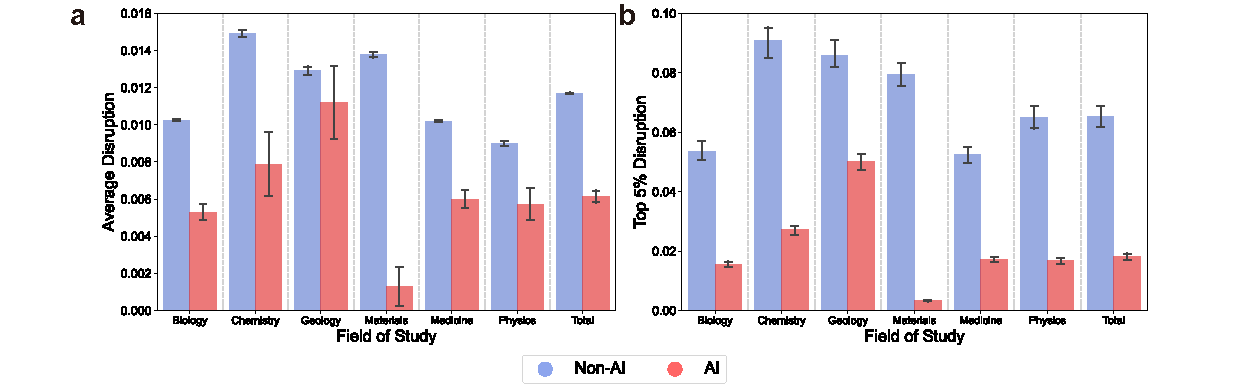
\includegraphics[width=\textwidth]{figure_SI/R1S7.pdf}
\caption{
\textbf{Comparison of disruption between AI and non-AI papers.}
\textbf{(a)} Average disruption of AI and non-AI papers in each field ($p<0.001, n=23,199,583$).
\textbf{(b)} Top 5th-percentile disruption of AI and non-AI papers in each field ($p<0.001, n=23,199,583$).
99\% CIs are shown as error bars centred at the mean or the 5\% percentile.
All statistical tests use a two-sided t-test.
}
\label{figsR1S7}
\end{figure}

\clearpage
\newpage
\begin{figure}[ht]
\centering
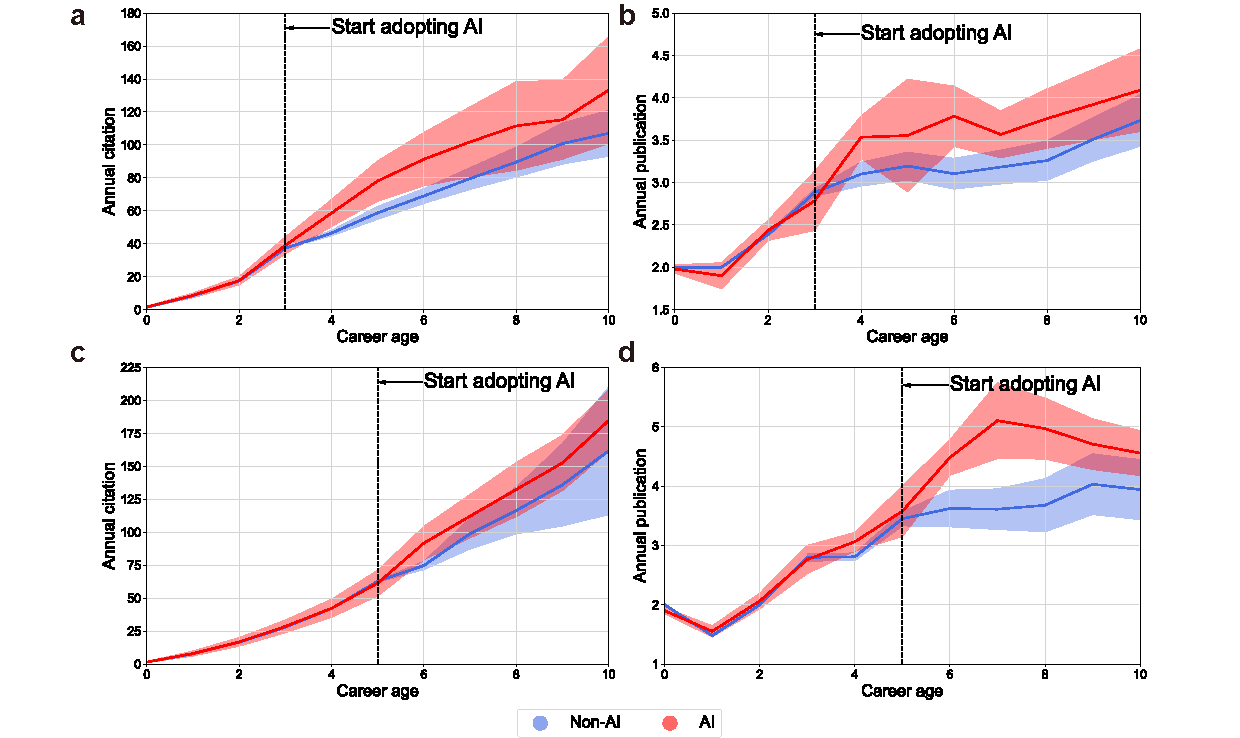
\includegraphics[width=\textwidth]{figure_SI/R1S11.pdf}
\caption{
\textbf{Match-and-comparison analysis on the role of AI in driving the advantages of scientific in productivity and scholarly impact.}
\textbf{(a)} Comparison between scientists who began adopting AI in the third year of their careers and matched counterparts who exhibited comparable annual citation counts during their first three years but never adopted AI.
\textbf{(b)} Comparison between scientists who began adopting AI in the third year of their careers and matched counterparts who exhibited comparable annual productivity during their first three years but never adopted AI.
\textbf{(c)} Comparison between scientists who began adopting AI in the fifth year of their careers and matched counterparts who exhibited comparable annual citation counts during their first three years but never adopted AI.
\textbf{(d)} Comparison between scientists who began adopting AI in the fifth year of their careers and matched counterparts who exhibited comparable annual productivity during their first three years but never adopted AI.
The results suggest that for scientists with comparable early-career positions, adopting AI itself contributes to their subsequent advantages in productivity and scholarly impact.
For all panels, 99\% CIs are shown as error bands centred at the mean.
}
\label{figsR1S11}
\end{figure}

\clearpage
\newpage
\begin{figure}[ht]
\centering
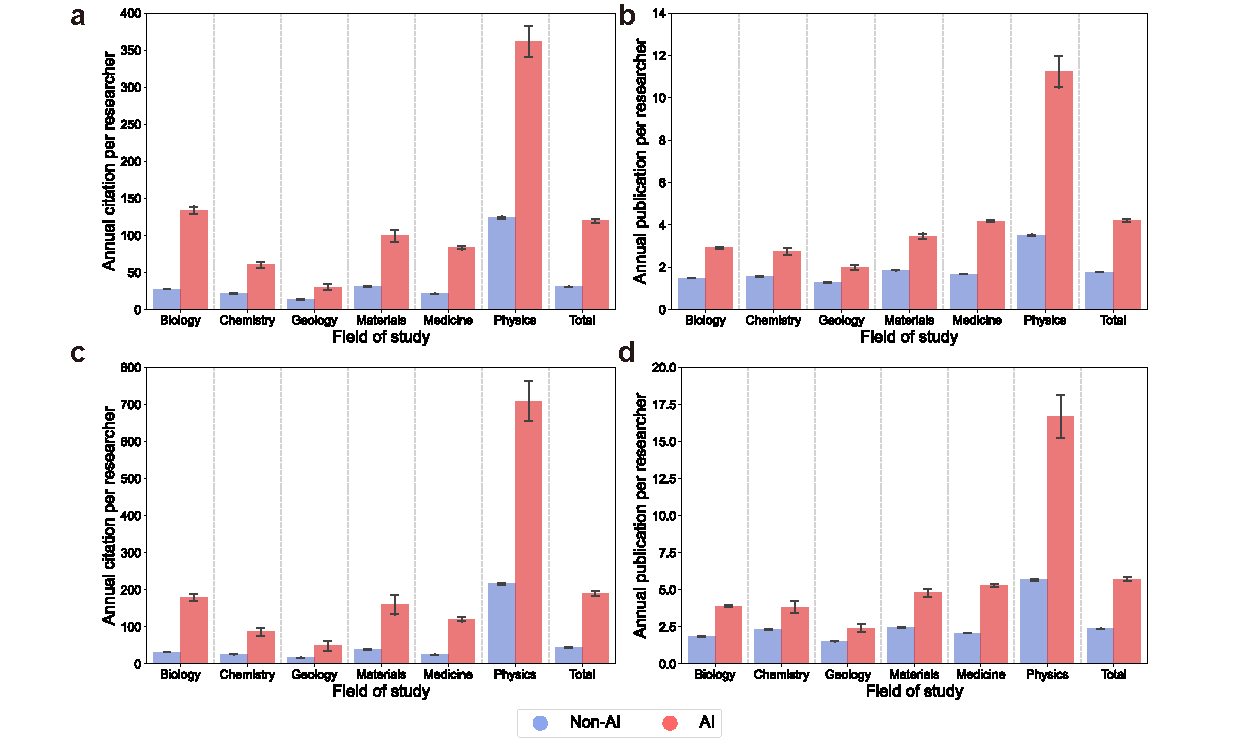
\includegraphics[width=\textwidth]{figure_SI/R1S6.pdf}
\caption{
\textbf{The impact of AI on the productivity and citation of researchers with multi-year continuous publication records.}
\textbf{(a)} Comparison of annual citations between researchers adopting AI and their counterparts without AI among those with at least five consecutive years of publications ($p<0.001, n=1,495,265$).
\textbf{(b)} Comparison of annual publications between researchers adopting AI and their counterparts without AI among those with at least five consecutive years of publications ($p<0.001, n=1,495,265$).
\textbf{(c)} Comparison of annual citations between researchers adopting AI and their counterparts without AI among those with at least ten consecutive years of publications ($p<0.001, n=525,716$).
\textbf{(d)} Comparison of annual publications between researchers adopting AI and their counterparts without AI among those with at least ten consecutive years of publications ($p<0.001, n=525,716$).
These results confirm the positive impact of AI adoption on the career progression of continuously publishing core scientists.
For all panels, 99\% CIs are shown as error bars centred at the mean.
All statistical tests use a two-sided t-test.
}
\label{figsR1S6}
\end{figure}

\clearpage
\newpage
\begin{figure}[ht]
\centering
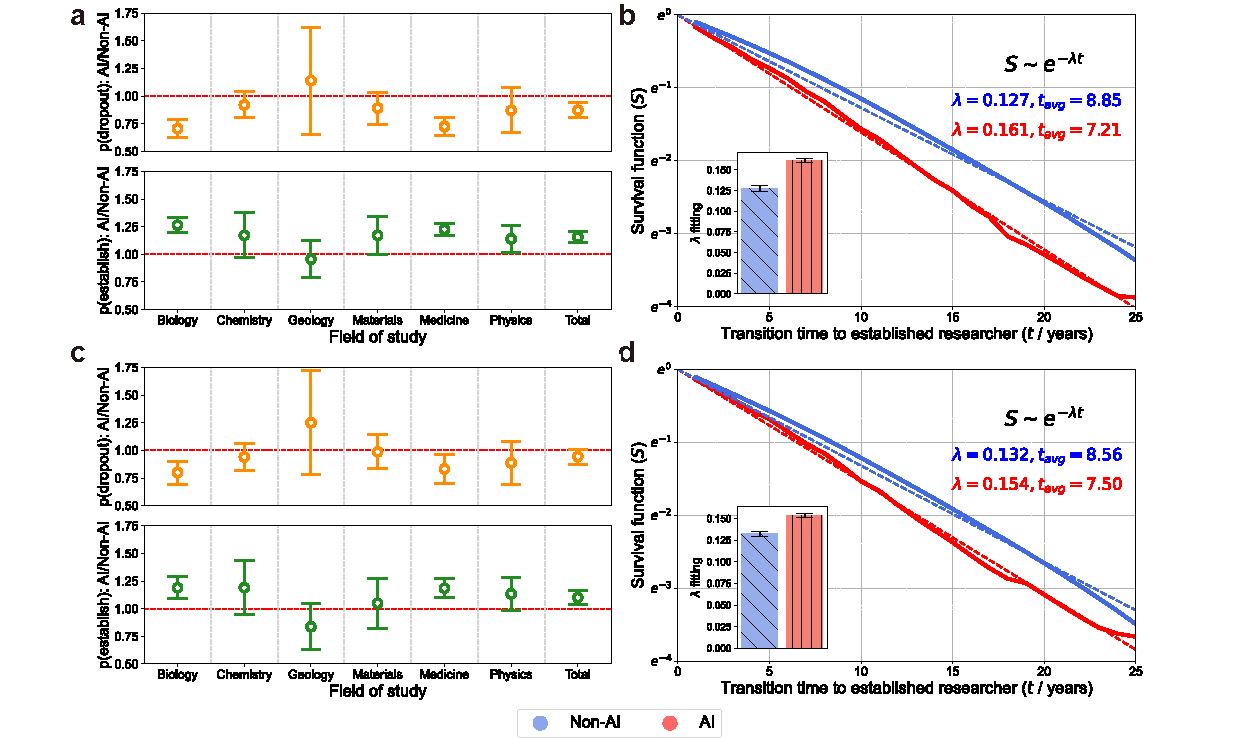
\includegraphics[width=\textwidth]{figure_SI/R1S2b.pdf}
\caption{
\textbf{Impact of AI adoption on researchers’ careers with different thresholds in detecting the dropout of researchers.}
\textbf{(a) (c)} The probability of two role transitions between junior scientists adopting AI and their counterparts without AI ($n=46$ year observations for each field).
\textbf{(b) (d)} Survival functions for the transition from junior to established researcher (b, $p<0.001, n=2,858,901$; d, $p<0.001, n=1,947,315$).
In (a) and (b), the threshold for detecting researcher dropout is 2 years.
In (c) and (d), the threshold for detecting researcher dropout is 4 years.
Results are consistent for both shorter and longer thresholds.
For all panels, 99\% CIs are shown as error bars centred at the mean.
All statistical tests use a two-sided t-test.
}
\label{figsR1S2b}
\end{figure}

\clearpage
\newpage
\begin{figure}[ht]
\centering

\includegraphics[width=\textwidth]{figure_SI/R1S2a.pdf}
\caption{
\textbf{The distribution of gap year durations in researcher’s careers.}
A period of gap years refers to a temporary interruption in a researcher’s publication activity, followed by a subsequent resumption of publishing. Results show that 44.67\% of all gap periods lasted only one year, and 76.94\% lasted no more than three years.
}
\label{figsR1S2a}
\end{figure}


\clearpage
\newpage
\begin{figure}[ht]
\centering
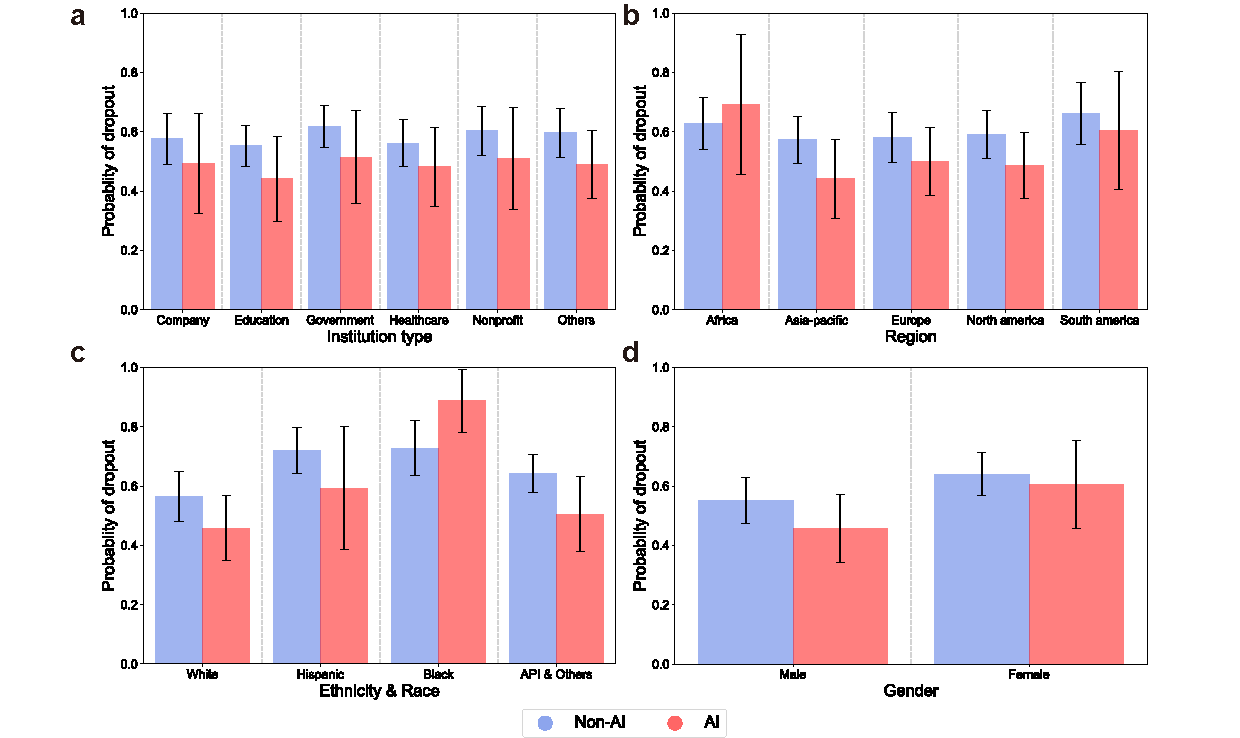
\includegraphics[width=\textwidth]{figure_SI/R1S10.pdf}
\caption{
\textbf{Impact of AI adoption on research careers across different demographic groups.}
\textbf{(a)} Researchers affiliated with institutions of different types ($n=2,140,845$).
\textbf{(b)} Researchers affiliated with institutions within different geographic regions ($n=2,140,845$).
\textbf{(c)} Researchers of different ethnicity and race ($n=1,438,544$).
\textbf{(d)} Researchers of different genders ($n=502,336$).
Results show the heterogeneous impact of AI on scientific careers across different demographic groups. 
For all panels, 99\% CIs are shown as error bars centred at the mean.
}
\label{figsR1S10}
\end{figure}


\clearpage
\newpage
\begin{figure}[ht]
\centering
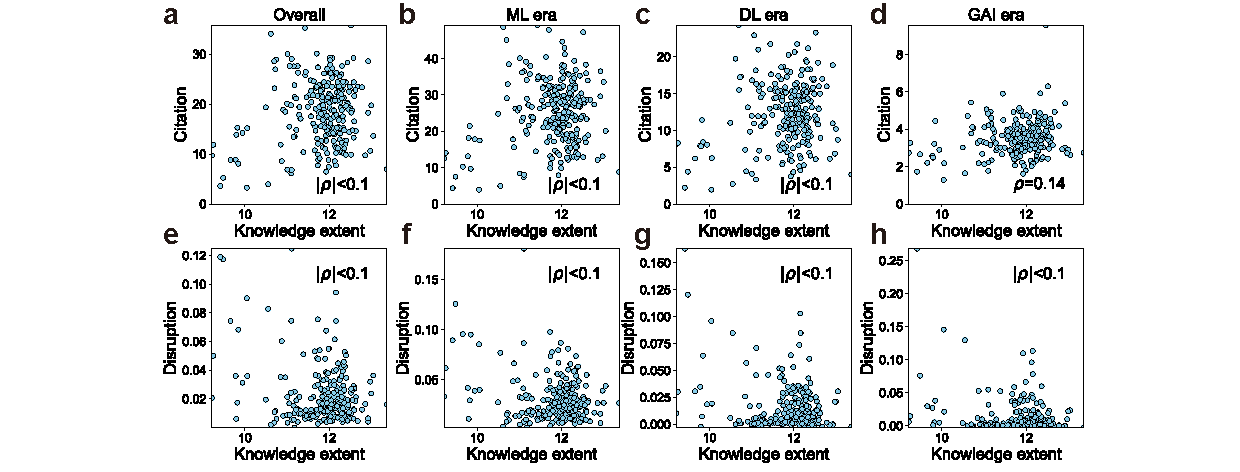
\includegraphics[width=\textwidth]{figure_SI/R1S1.pdf}
\caption{
\textbf{Correlation analysis between knowledge extent and citation or disruption of sub-fields.}
For all panels, each scatter represents a sub-field, and the corresponding Pearson’s $r$ is indicated correspondingly.
Results show that, across sub-fields and eras of AI development, neither citation impact (as a proxy for impact) nor disruption (as a proxy for novelty) is obviously correlated with the sub-field’s knowledge extent.
}
\label{figsR1S1}
\end{figure}


\clearpage
\newpage
\begin{figure}[ht]
\centering

\includegraphics[width=\textwidth]{figure_SI/R1S15a.pdf}
\caption{
\textbf{Selectivity of AI adoption in different topics regarding topicality itself.}
The citation relationships between AI and non-AI papers show that AI research across various fields is more frequently cited by non-AI studies than by AI studies themselves ($p<0.001, n=27,405,011$).
This suggests that topics in AI research influence non-AI research rather than forming isolated, self-referential clusters of AI literature.
There tends to be no obvious difference in topic selection between AI and non-AI research, indicating that inherent topicality does not account for the observed more narrow focus of AI-augmented research.
99\% CIs are shown as error bars centred at the mean, and the statistical tests use a two-sided t-test.
}
\label{figsR1S15a}
\end{figure}


\clearpage
\newpage
\begin{figure}[ht]
\centering
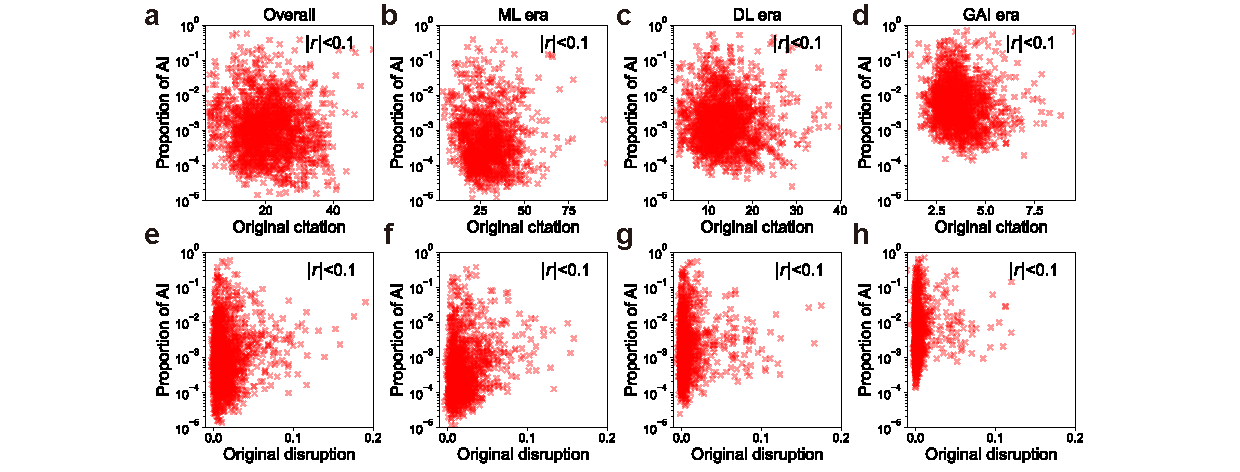
\includegraphics[width=\textwidth]{figure_SI/R1S15b.pdf}
\caption{
\textbf{Selectivity of AI adoption in different topics associated with the topics’ original impact.}
In all panels, each scatter shows the degree of AI penetration in a topic and the original citation count or disruption score within that topic.
The corresponding Pearson’s $r$ is indicated in each panel.
Results show that across topics and AI eras, neither the original citation nor the original disruption is obviously correlated with the proportion of AI adoption, suggesting that AI adoption does not selectively favor topics based on differential original impact.
}
\label{figsR1S15b}
\end{figure}


\clearpage
\newpage
\begin{figure}[ht]
\centering
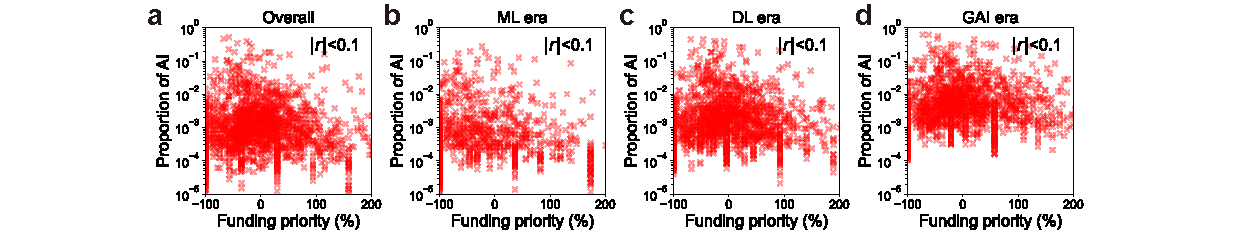
\includegraphics[width=\textwidth]{figure_SI/R1S15c.pdf}
\caption{
\textbf{Selectivity of AI adoption in different topics regarding funding priority across the topics.}
In all panels, each scatter shows the degree of AI penetration in a topic and funding priority to that topic.
The corresponding Pearson’s $r$ is indicated correspondingly in each panel. 
Results show that across topics and AI eras, there are heterogeneous funding priorities for different topics, but funding priority is not obviously correlated with the proportion of AI adoption, suggesting that AI adoption does not selectively favor topics prioritized by funding agencies.
}
\label{figsR1S15c}
\end{figure}


\clearpage
\newpage
\begin{figure}[ht]
\centering
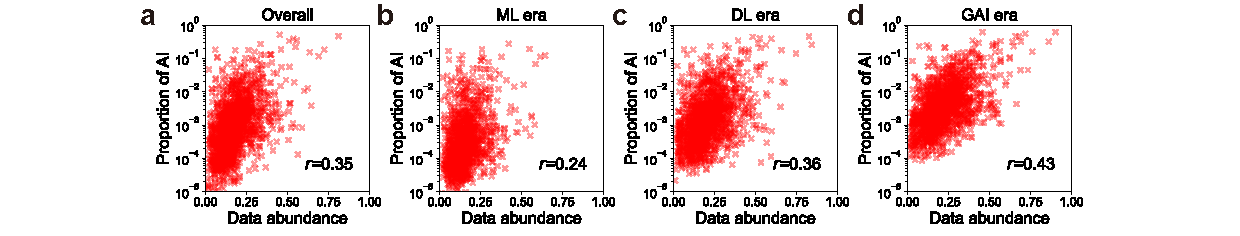
\includegraphics[width=\textwidth]{figure_SI/R1S15d.pdf}
\caption{
\textbf{Selectivity of AI adoption in different topics regarding data abundance in the topics.}
In all panels, each scatter shows the degree of AI penetration in a topic and the data abundance in that topic.
The corresponding Pearson’s $r$ is indicated correspondingly in each panel. The results show that across topics and AI eras, the data abundance is positively correlated with the proportion of AI adoption, suggesting that AI is more likely to be adopted in topics with abundant data resources.
Notably, the correlation of AI-use with frequency of mentioned data resources rises with the size and intensity of AI-models.
}
\label{figsR1S15d}
\end{figure}


\clearpage
\newpage
\begin{figure}[ht]
\centering
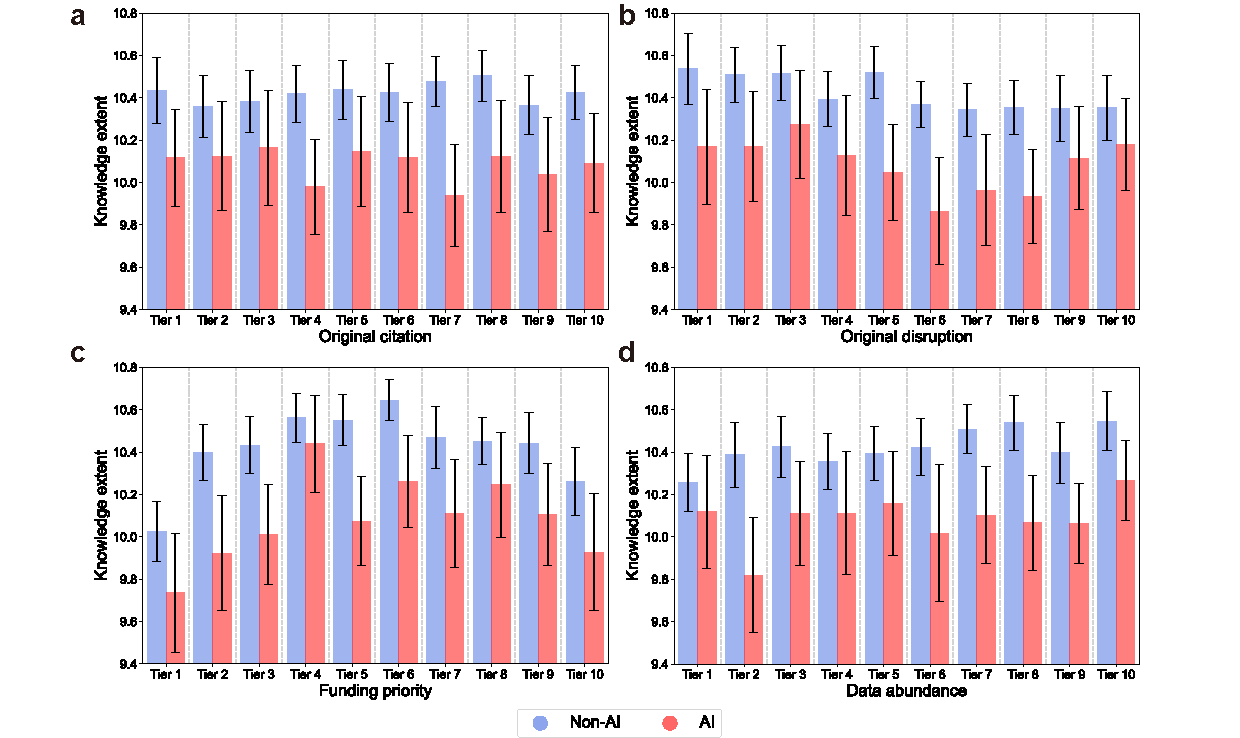
\includegraphics[width=\textwidth]{figure_SI/R1S16.pdf}
\caption{
\textbf{Stratified analyses controlling for the effects of potential confounding variables on the contracted knowledge extent of AI-augmented research.}
The results show that when dividing each external factor into 10 tiers based on magnitude, the contraction in knowledge extent for AI-augmented research remains evident within each tier ($p<0.001, n=17,529,094$).
Therefore, regardless of whether a topic is more or less likely to be selected for AI adoption, existing AI-augmented research within the topic consistently covers a contracted knowledge space compared to non-AI research.
For all panels, 99\% CIs are shown as error bars centred at the mean.
All statistical tests use a two-sided t-test.
}
\label{figsR1S16}
\end{figure}


\clearpage
\newpage
\begin{figure}[ht]
\centering
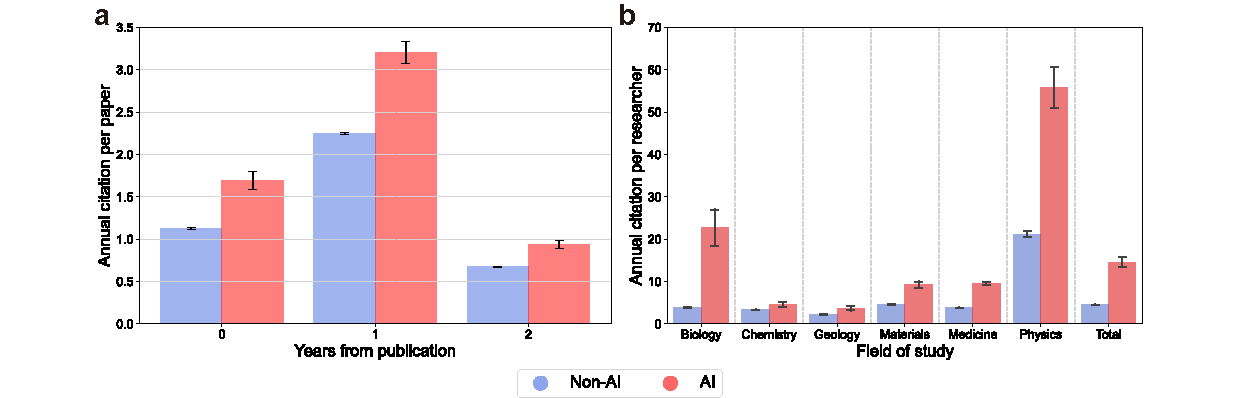
\includegraphics[width=\textwidth]{figure_SI/LLMera2.pdf}
\caption{
\textbf{Replication of “AI enlarges the impact of papers” with only the subset of papers published during the GAI era.}
\textbf{(a)} Annual citations after publication of AI and non-AI papers ($n=1,888,694$).
\textbf{(b)} Average annual citations of researchers adopting AI and their counterparts without AI ($p<0.001, n=2,888,737$).
For all panels, 99\% CIs are shown as error bars centred at the mean.
All statistical tests use a two-sided t-test.
Results in the GAI era are consistent with those obtained over the full time span featured in the main text.
}
\label{figLLMera2}
\end{figure}

\clearpage
\newpage
\begin{figure}[ht]
\centering
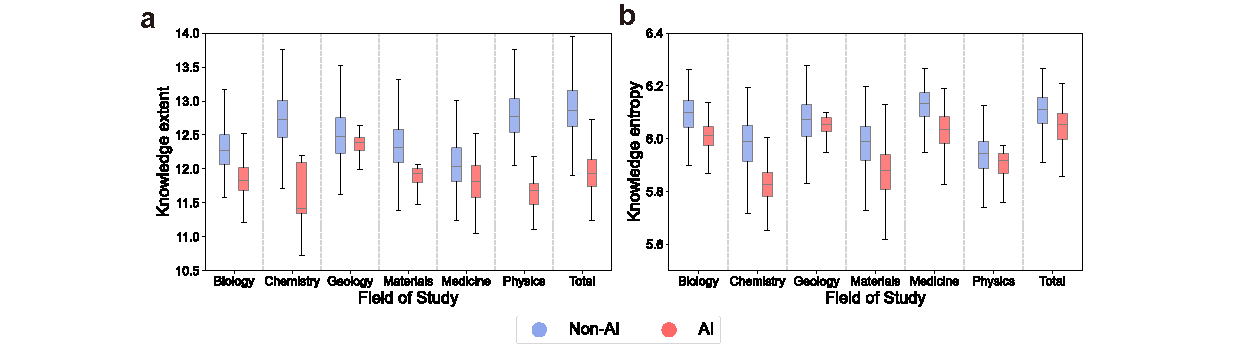
\includegraphics[width=\textwidth]{figure_SI/LLMera3.pdf}
\caption{
\textbf{Replication of “AI usage is associated with a contraction in knowledge extent within and across scientific fields” with only the subset of papers published during the GAI era.}
\textbf{(a)} Knowledge extent of AI and non-AI papers in each field ($n=1,000$ samples in each field).
\textbf{(b)} Knowledge entropy of AI and non-AI papers in each field ($n=1,000$ samples in each field).
Boxplots are centred at the median and bounded at the first and third quartile (Q1 and Q3), with 1.5 times of the inter-quartile range (IQR) shown as whiskers from the box.
Results in the GAI era are consistent with those obtained over the full time span featured in the main text.
}
\label{figLLMera3}
\end{figure}

\clearpage
\newpage
\begin{figure}[ht]
\centering
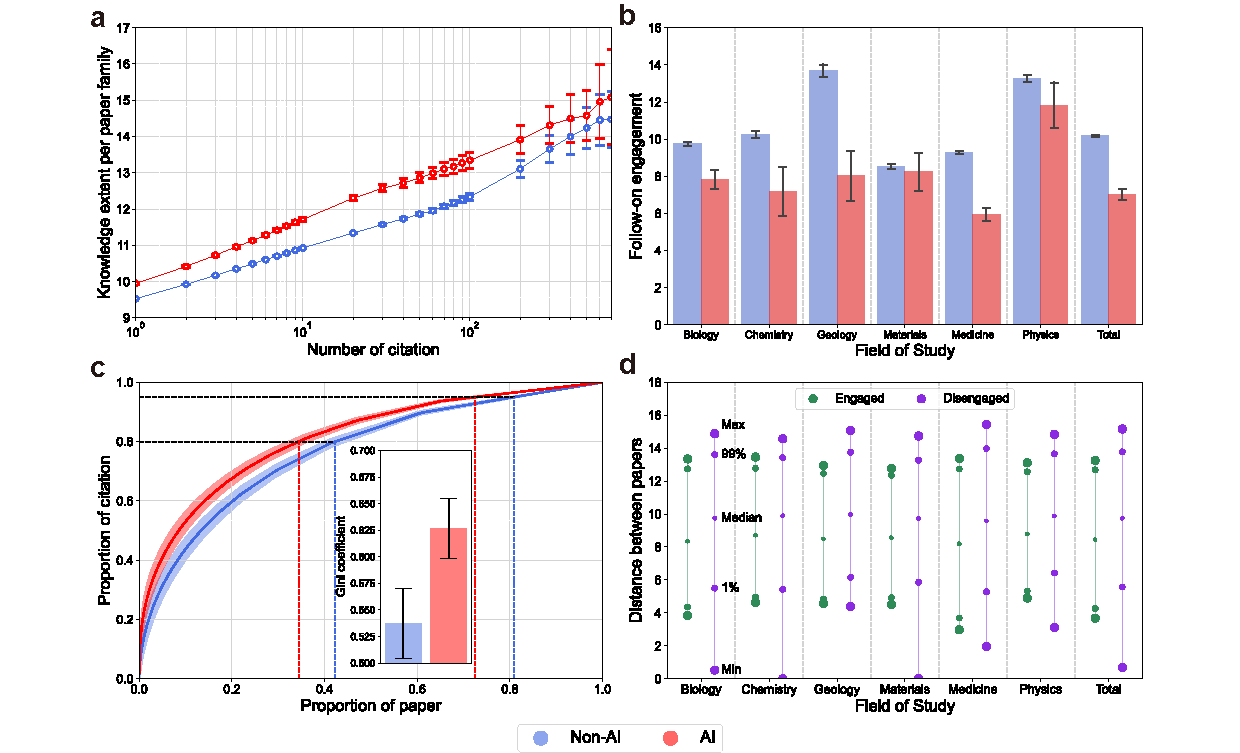
\includegraphics[width=\textwidth]{figure_SI/LLMera4.pdf}
\caption{
\textbf{Replication of “reduced follow-on engagement and more overlapped works in AI research” with only the subset of papers published during the GAI era.}
\textbf{(a)} Knowledge extent of individual AI and non-AI paper families ($n=1,888,694$).
\textbf{(b)} Engagement among papers that cite AI vs. non-AI papers ($p<0.001, n=518,156$).
\textbf{(c)} Distribution of citations to AI vs. non-AI papers ($p<0.001, n=100$ sampled paper groups).
\textbf{(d)} Distribution of distances between paper pairs that cite the same papers, with or without citing each other—engaged versus disengaged ($n=258,529$ sampled paper pairs).
For all panels, 99\% CIs are shown as error bars or error bands centred at the mean.
All statistical tests use a two-sided t-test.
Results in the GAI era are consistent with those on the full time span featured in the main text.
}
\label{figLLMera4}
\end{figure}

\clearpage
\newpage
\begin{figure}[ht]
\centering
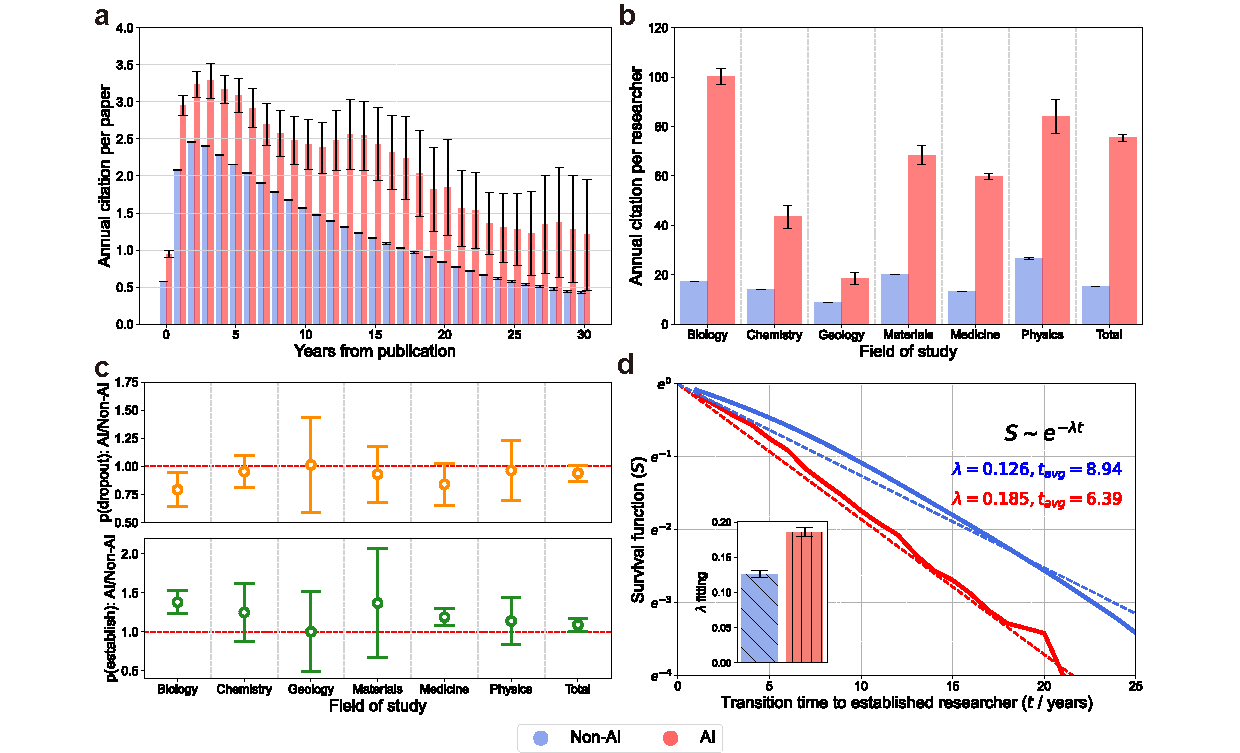
\includegraphics[width=\textwidth]{figure_SI/WoS2.pdf}
\caption{
\textbf{Replication of “AI enlarges the impact of papers and enhances the career of researchers” on the WOS dataset.}
\textbf{(a)} Annual citations after publication of AI and non-AI papers ($n=16,706,988$).
\textbf{(b)} Average annual citations of researchers adopting AI and their counterparts without AI ($p<0.001, n=3,620,795$).
\textbf{(c)} The probability of two role transitions between junior scientists adopting AI and their counterparts without AI ($n=46$ year observations for each field).
\textbf{(d)} Survival functions for the transition from junior to established researcher ($p<0.001, n=1,556,338$).
For all panels, 99\% CIs are shown as error bars centred at the mean.
All statistical tests use a two-sided t-test.
Results on the WOS dataset are consistent with those from the OpenAlex dataset featured in the main text.
}
\label{figWoS2}
\end{figure}

\clearpage
\newpage
\begin{figure}[ht]
\centering
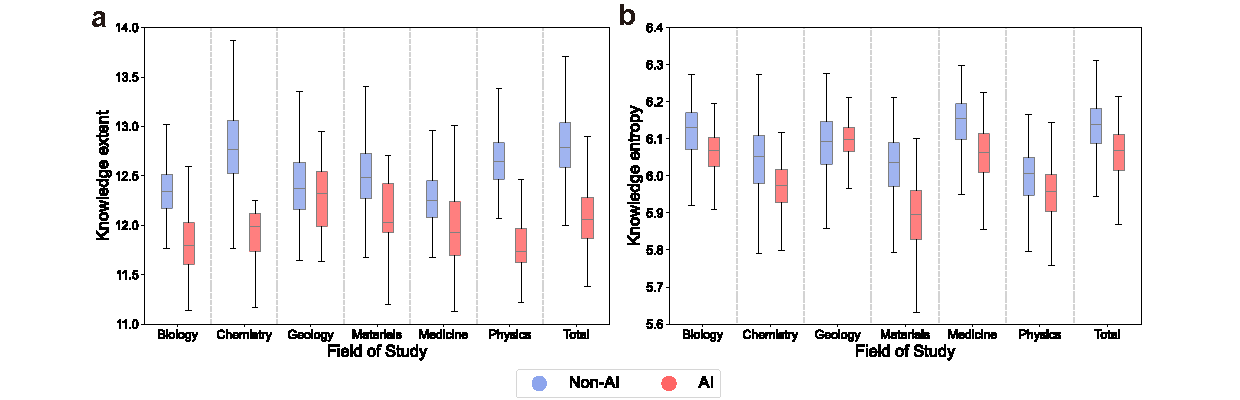
\includegraphics[width=\textwidth]{figure_SI/WoS3.pdf}
\caption{
\textbf{Replication of “AI usage is associated with a contraction in knowledge extent within and across scientific fields” on the WOS dataset.}
\textbf{(a)} Knowledge extent of AI and non-AI papers in each field ($n=1,000$ samples in each field).
\textbf{(b)} Knowledge entropy of AI and non-AI papers in each field ($n=1,000$ samples in each field).
Boxplots are centred at the median and bounded at the first and third quartile (Q1 and Q3), with 1.5 times of the inter-quartile range (IQR) shown as whiskers from the box.
Results on the WOS dataset are consistent with the ones on OpenAlex featured in the main text.
}
\label{figWoS3}
\end{figure}

\clearpage
\newpage
\begin{figure}[ht]
\centering
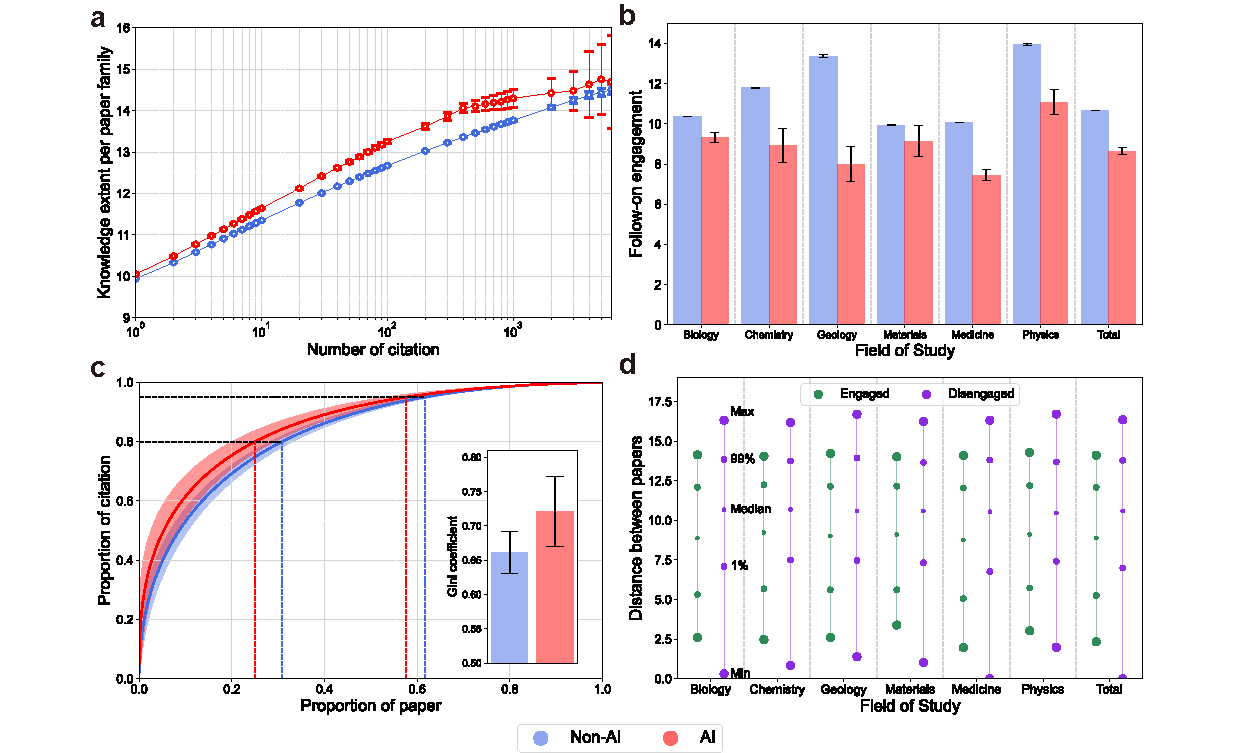
\includegraphics[width=\textwidth]{figure_SI/WoS4.pdf}
\caption{
\textbf{Replication of “reduced follow-on engagement and more overlapped works in AI research” on the WOS dataset.}
\textbf{(a)} Knowledge extent of individual AI and non-AI paper families ($n=16,706,988$).
\textbf{(b)} Engagement among papers that cite AI vs. non-AI papers ($p<0.001, n=15,048,254$).
\textbf{(c)} The distribution of citations to AI vs. non-AI papers ($p<0.001, n=100$ sampled paper groups).
\textbf{(d)} The distribution of distances between paper pairs that cite the same papers, with or without citing each other—engaged versus disengaged ($n=674,132,352$ sampled paper pairs).
For all panels, 99\% CIs are shown as error bars or error bands centred at the mean.
All statistical tests use a two-sided t-test.
Results from the WOS dataset are consistent with those from the OpenAlex dataset featured in the main text.
}
\label{figWoS4}
\end{figure}

\clearpage
\newpage
\begin{figure}[ht]
\centering
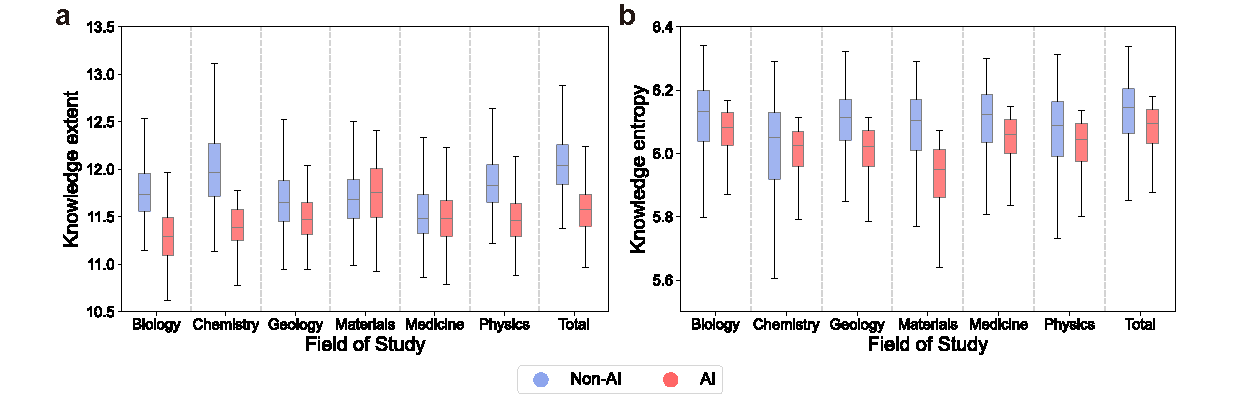
\includegraphics[width=\textwidth]{figure_SI/R2S1a.pdf}
\caption{
\textbf{Replication of “AI usage is associated with a contraction in knowledge extent within and across scientific fields” in an embedding space after dimensional reduction using PCA.}
\textbf{(a)} Knowledge extent of AI and non-AI papers in each field ($n=1,000$ samples in each field).
\textbf{(b)} Knowledge entropy of AI and non-AI papers in each field ($n=1,000$ samples in each field).
Boxplots are centred at the median and bounded at the first and third quartile (Q1 and Q3), with 1.5 times of the inter-quartile range (IQR) shown as whiskers from the box.
Results in the reduced-dimensional space are consistent with those from the original embedding space reported in the main text.
}
\label{figsR2S1a}
\end{figure}

\clearpage
\newpage
\begin{figure}[ht]
\centering
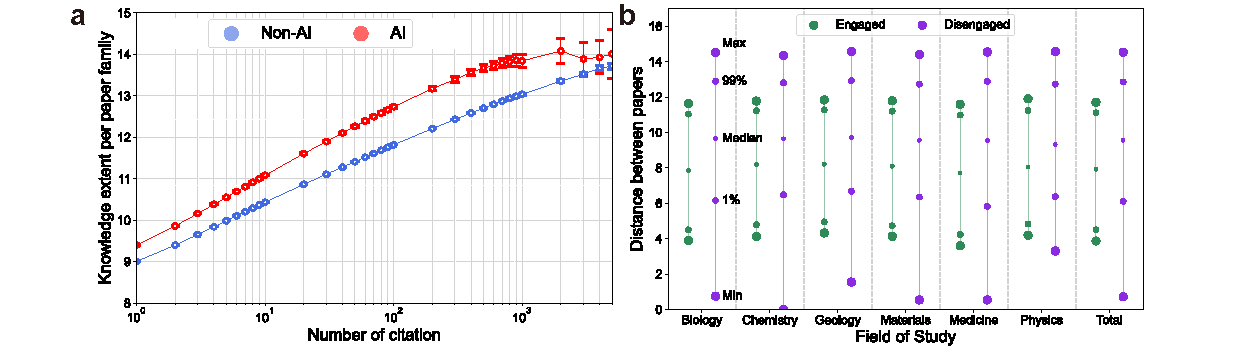
\includegraphics[width=\textwidth]{figure_SI/R2S1b.pdf}
\caption{
\textbf{Replication of “reduced follow-on engagement and more overlapped works in AI research” in an embedding space after dimensional reduction using PCA.}
\textbf{(a)} Knowledge extent of individual AI and non-AI paper families ($n=27,405,011$).
99\% CIs are shown as error bars centred at the mean.
\textbf{(b)} The distribution of distances between paper pairs that cite the same papers, with or without citing each other—engaged versus disengaged ($n=590,325,130$ sampled paper pairs).
Results in the reduced-dimensional space are consistent with those from the original embedding space reported in the main text.
}
\label{figsR2S1b}
\end{figure}

\clearpage
\newpage
\begin{figure}[ht]
\centering
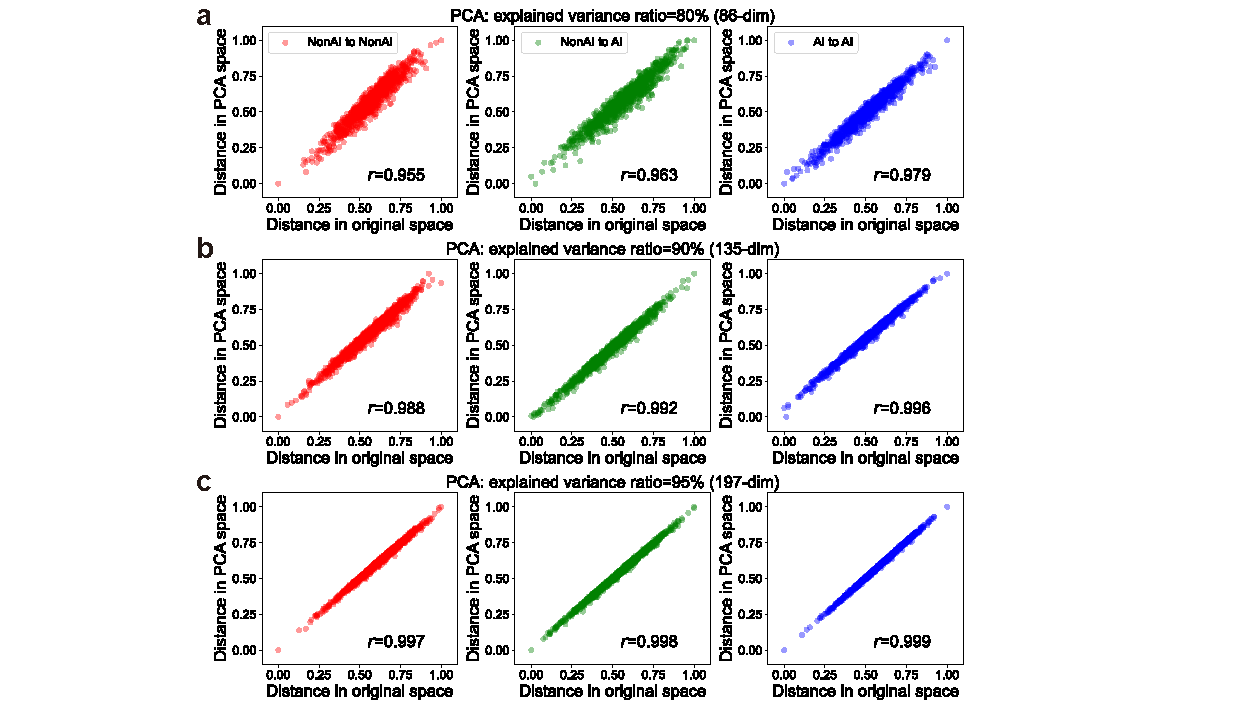
\includegraphics[width=\textwidth]{figure_SI/R2S2.pdf}
\caption{
\textbf{General sensitivity check on the distance calculations in high-dimensional paper embedding space.}
We reduce the original embeddings to 86, 135, and 197 dimensions with PCA, which correspond to the principal components that explain \textbf{(a)} 80\%, \textbf{(b)} 90\%, and \textbf{(c)} 95\% of the total variance, respectively.
We then randomly sampled 1,000 NonAI-NonAI, 1,000 AI-AI, and 1,000 NonAI-AI paper pairs and calculated the distance for each pair within each of the reduced-dimensional spaces.
Results show that the distances in the various reduced-dimensional spaces are highly correlated with those in the original space, indicating the reliability of our paper embeddings for distance calculations.
}
\label{figsR2S2}
\end{figure}

\clearpage
\newpage
\begin{figure}[ht]
\centering
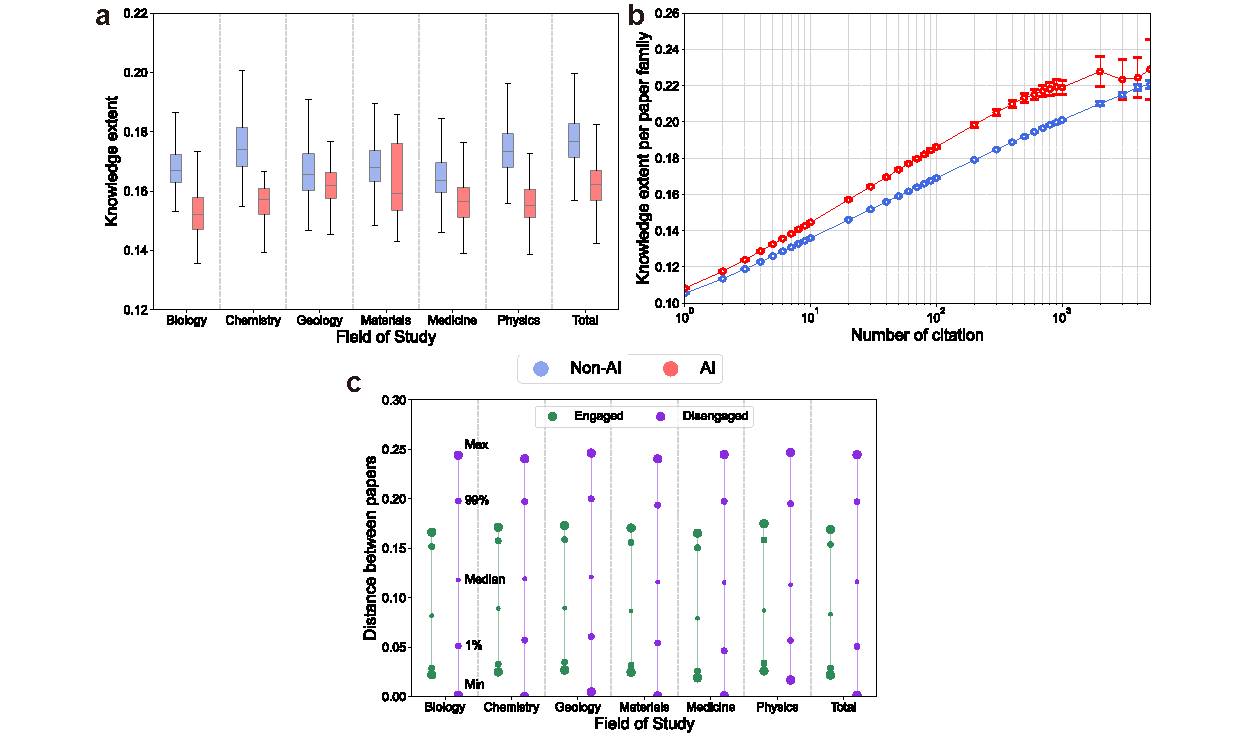
\includegraphics[width=\textwidth]{figure_SI/R2S5.pdf}
\caption{
\textbf{Replication of results related to high-dimensional distance calculations with Cosine distance.}
\textbf{(a)} Knowledge extent of AI and non-AI papers in each field ($n=1,000$ samples in each field).
Boxplots are centred at the median and bounded at the first and third quartile (Q1 and Q3), with 1.5 times of the inter-quartile range (IQR) shown as whiskers from the box.
\textbf{(b)} Knowledge extent of individual AI and non-AI paper families ($n=27,405,011$).
99\% CIs are shown as error bars centred at the mean.
\textbf{(c)} The distribution of distances between paper pairs that cite the same papers, with or without citing each other-engaged versus disengaged ($n=590,325,130$ sampled paper pairs).
Results with Cosine distance are consistent with those with Euclidean distance reported in the main text.
}
\label{figsR2S5}
\end{figure}